% autore: Andrea Ciprietti

    \createsection{\BottomUp}{{\small{$\blacksquare$}} \normalsize Approccio \textit{bottom-up}}
    \createsection{\TopDown}{{\small{$\blacksquare$}} \normalsize Approccio \textit{top-down}}
    \createsection{\Codice}{{\small{$\blacksquare$}} \normalsize Codice della soluzione}
    
    Si tratta di una variante del ben noto problema dello zaino (o \textit{knapsack problem}), in cui si richiede di determinare -- dati diversi tipi di oggetti cui sono associati un peso (intero) e un valore -- l'insieme di oggetti (anche più di uno per ciascun tipo) il cui peso non superi un certo tetto e la cui somma dei valori sia massima.

    Nel nostro caso, invece, sono dati in input un insieme di $N$ portate -- ciascuna avente un proprio peso -- e un intero $K$, e viene chiesto di determinare il sottoinsieme di peso minimo non inferiore a $K$. Si noti che, a differenza del problema dello zaino, quello che cerchiamo è un valore minimo (e non un massimo); inoltre, è possibile prendere alpiù una protata per ogni tipo, e il valore di ciascuna di esse coincide con il suo peso.
    
    Per risolvere il problema si sfrutterà la tecnica della programmazione dinamica (abbreviata anche in \textit{DP}, \textit{dynamic programming}). Di seguito, proponiamo e illustriamo due approcci formalmente diversi, ma sostanzialmente equivalenti per complessità computazionale e consumo di memoria: quello \textit{bottom-up} e quello \textit{top-down}.
    
    \BottomUp
    
    L'idea centrale della DP sta nel suddividere il problema iniziale in tanti sottoproblemi, dipendenti da uno o più parametri (in questo caso, l'insieme delle portate e il peso minimo), in modo che sia possibile risolvere ogni sottoproblema a partire dalle soluzioni intermedie di casi più semplici. Le soluzioni dei sottoproblemi vengono ``immagazzinate'' (in gergo, memoizzate) in una tabella (che può essere un array o -- più in generale -- una matrice $k$-dimensionale, dove $k$ sono i parametri da cui dipendono i sottoproblemi) e usati per ``ricostruire'' la soluzione del problema vero e proprio.
    
    \begin{wrapfigure}{r}{.25\textwidth}
        \vspace*{-.9cm}
        \begin{flushright}
            \asyinclude{asy_nonna/fig1_a.asy}
        \end{flushright}
        \vspace*{-.5cm}
    \end{wrapfigure}
    
    La tecnica \textit{bottom-up} consiste nel riempire la tabella dal basso, vale a dire partendo dai sottoproblemi più piccoli (cosiddetti casi base) e risolvere, uno dopo l'altro, i sottoproblemi via via più complessi. Nel caso in questione, costruiremo una matrice $N \times K$ per lo storaggio delle soluzioni: nella cella di coordinate $(i,j)$ manterremo la soluzione ottimale per il problema ridotto ai primi $i$ panini e a un peso totale minimo di $j$. Per calcolarla, basterà considerare le possibili scelte relative all'$i$-esima portata, e scegliere quella che porta a una soluzione globale minore:
    \begin{itemize}
    \item Se scegliamo di non mangiarla, allora ci riduciamo al sottoproblema con $i - 1$ portate e peso minimo $j$ che, per come viene costruita la tabella, è stato già risolto precedentemente.
    \item Se, al contrario, scegliamo di mangiarla, il sottoproblema cui ci riduciamo è quello con $i - 1$ portate e peso minimo $j - \texttt{P[$i - 1$]}$ (dove \texttt{P[$i - 1$]} è il peso dell'$i$-esima portata). Naturalmente, se $\texttt{P[$i - 1$]} > j$ la quantità $j - \texttt{P[$i - 1$]}$ è negativa, e non ha dunque una corrispondenza nella tabella. In questo caso, tuttavia, possiamo assumere che la soluzione ottima sia $0$ (intuitivamente, un peso totale nullo è comunque maggiore di un limite negativo).
    \end{itemize}
    
    Resta solo da risolvere ``a mano'' i casi base, ossia i sottoproblemi che non possono essere ricomposti: si tratta di quelli in cui il parametro $i$ è nullo -- in cui, cioè, non abbiamo a disposizione alcuna portata: è facile convincersi che, se $j = 0$, la soluzione ottima è $0$; per tutti gli altri valori di $j$ (da $1$ a $K$) possiamo convenzionalmente assegnare il valore fittizio $\infty$, sebbene in realtà non esista una soluzione.
    
    I sottoproblemi sono $N \cdot K$, e ognuno di essi viene risolto in tempo costante: la complessità asintotica dell'algoritmo è dunque pari a $O(N \cdot K)$.
    
    \TopDown
    
    La programmazione dinamica \textit{top-down} agisce esattamente come quella \textit{bottom-up}, risolvendo il problema iniziale a partire dai sottoproblemi, mediante la medesima relazione di ricorrenza e con gli stessi casi base. Tuttavia, stavolta la tabella viene riempita partendo ``dall'alto'', e riconducendosi ai sottoproblemi con opportune chiamate ricorsive. Le soluzioni intermedie, una volta calcolate per la prima volta, verranno ricordate in modo da non doverle ricomputare di nuovo successivamente. Per questo motivo, tale tecnica viene anche definita \textit{ricorsione con memoizzazione}.
    
    Come già detto, questo approccio ha, come il precedente, complessità e consumo di memoria $O(N \cdot K)$.
    
    \Codice
    
    Di seguito riportiamo l'implementazione della soluzione \textit{bottom-up} e di quella \textit{top-down}.
    
    \colorbox{white}{\makebox[.99\textwidth][l]{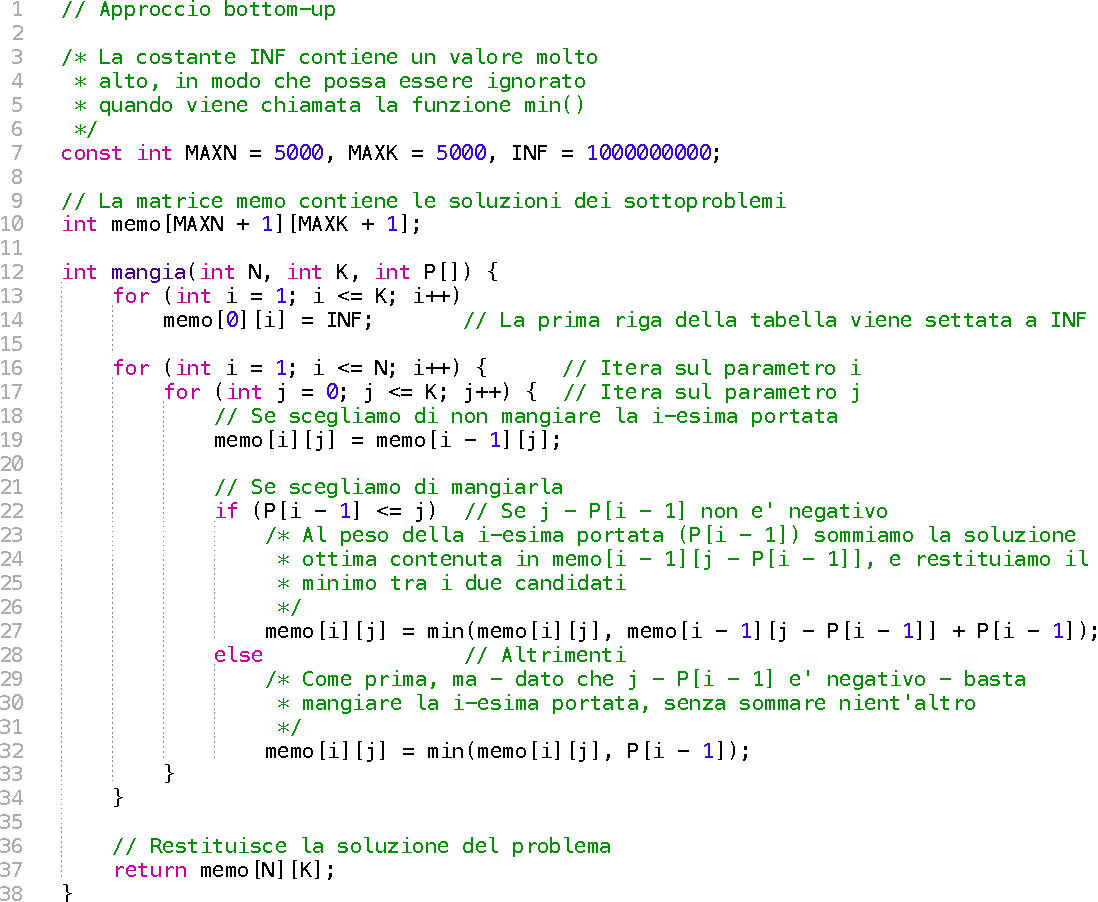
\includegraphics[scale=.8]{nonna_bu.pdf}}}
    
    \colorbox{white}{\makebox[.99\textwidth][l]{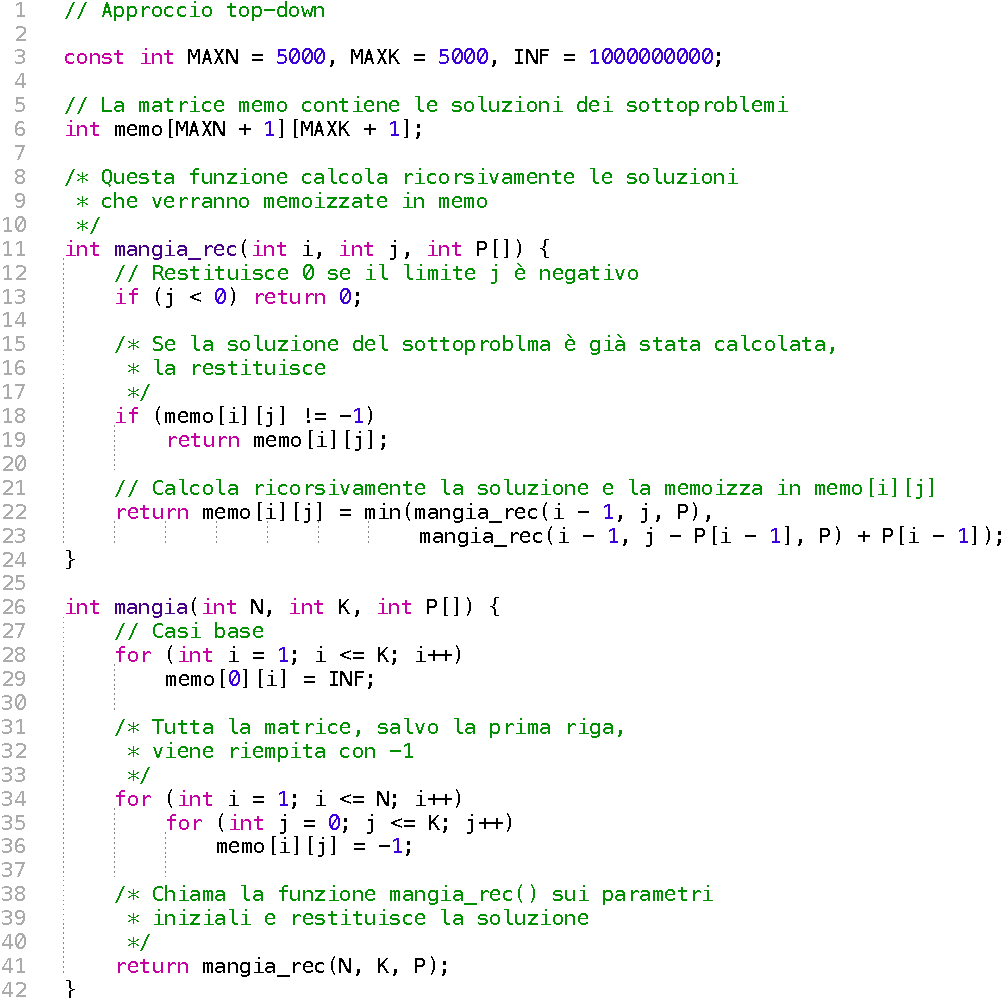
\includegraphics[scale=.8]{nonna_td.pdf}}}